% \section{Motivation}
% \label{sec:motivation}

% % Does adding a threat model section make sense?
% \amirian{Given the intro, I think we can safely remove this section. I've tried to work in pertinent parts into the intro}

% % but whatever works for lambdas is applicable to containers & VMs...
% % can we definitively say this?

\section{Methodology}
\label{sec:methodology}

% TODO: This figure shows only mem access latencies of exotic 
% operation. how does these operations affect latencies of other exotic 
% operations or regular memory accesses?
\begin{figure*}[h!]
\begin{subfigure}{.33\textwidth}
  \centering
  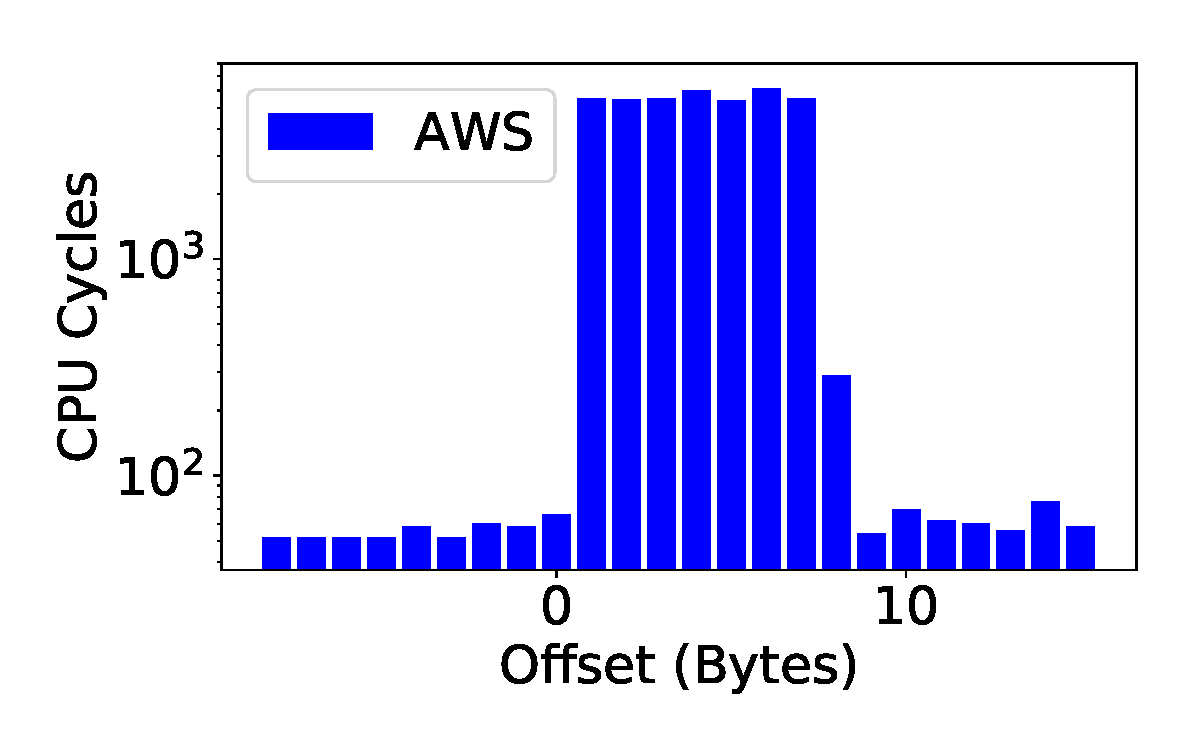
\includegraphics[width=.99\linewidth]{fig/membus_aws.pdf}
%   \caption{1a}
%   \label{fig:sfig1}
\end{subfigure}%
\begin{subfigure}{.33\textwidth}
  \centering
  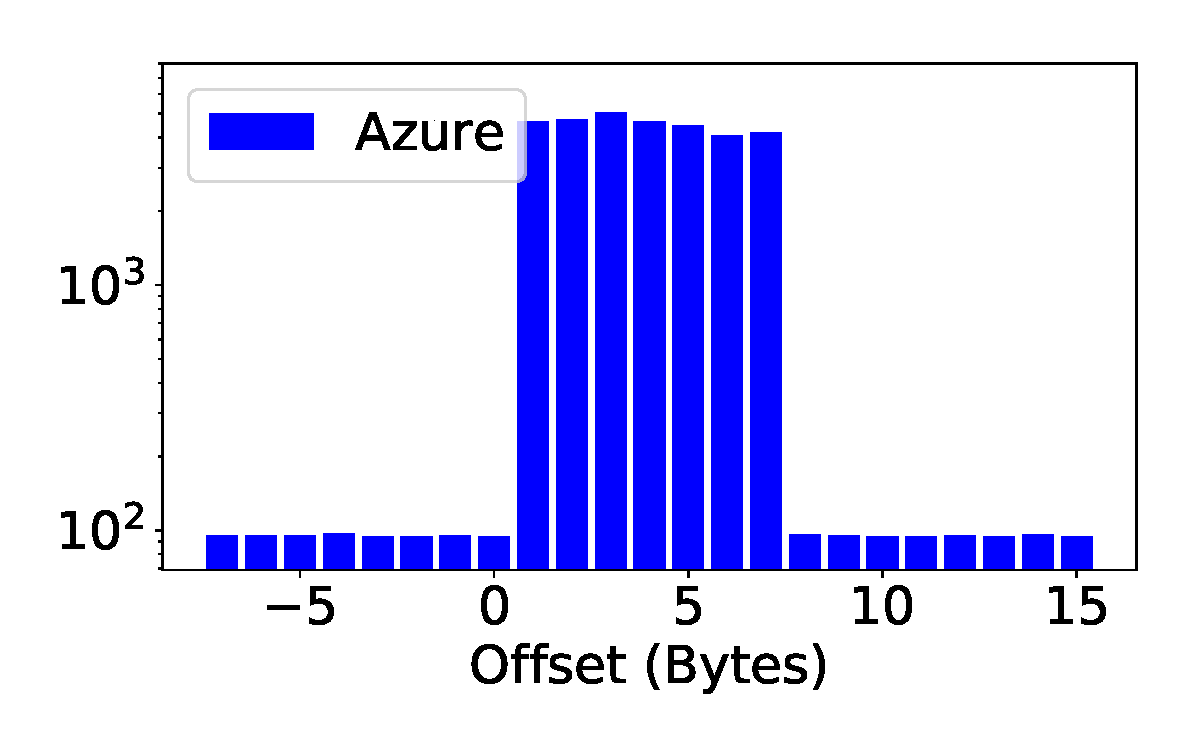
\includegraphics[width=.99\linewidth]{fig/membus_azure.pdf}
%   \caption{1b}
%   \label{fig:sfig2}
\end{subfigure}
\begin{subfigure}{.33\textwidth}
  \centering
  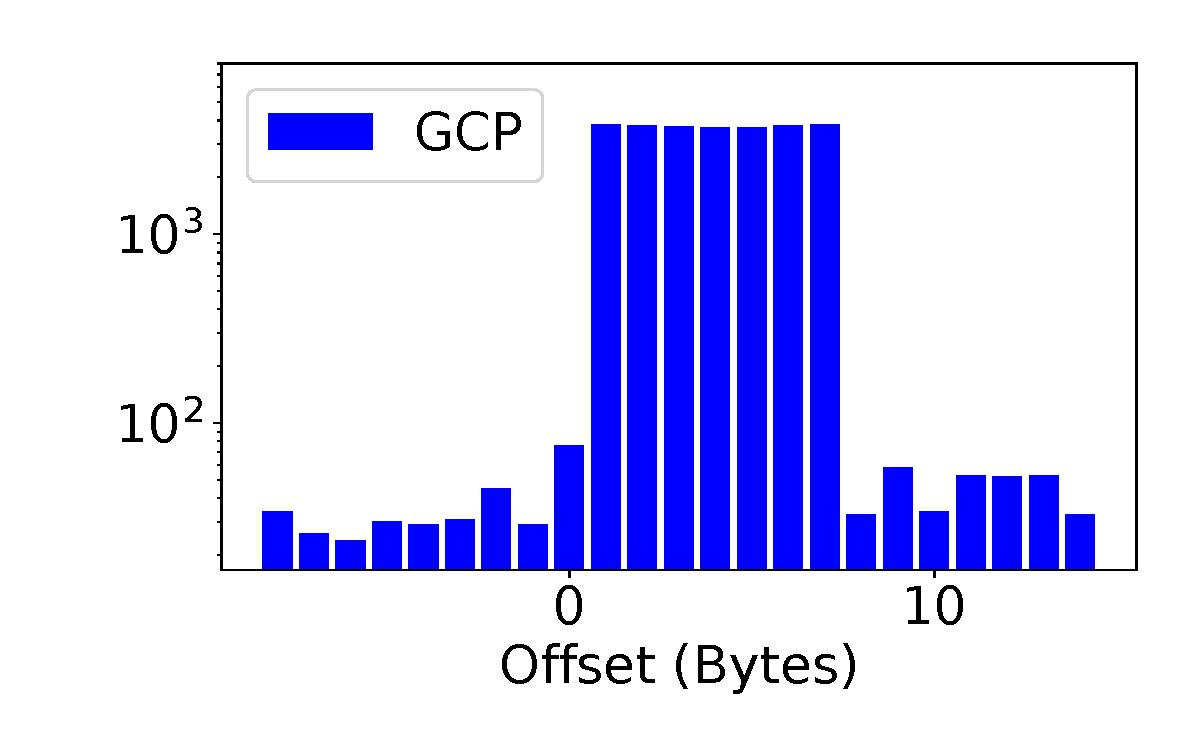
\includegraphics[width=.99\linewidth]{fig/membus_gcp.pdf}
%   \caption{1b}
%   \label{fig:sfig2}
\end{subfigure}
\caption{From left to right, the plots show the latencies of atomic 
      memory operations performed on an 8B memory region as we slide it 
      from one cache line across the boundary into another, on AWS, Azure and 
      Google (GCP) clouds respectively. The latencies 
      are orders of magnitude higher when the 8B region falls across the 
      two cache lines (offsets 0-7B) demonstrating the presence of 
      the memory bus covert channel on all these clouds. \label{fig:membus_clouds}}
\label{fig:fig}
\end{figure*}


Our goal is to determine a (co-operative) co-residence detection mechanism for
lambdas. In other words, given a series of spawned lambdas in a
certain region of a cloud service, how can we determine the lambdas that are
co-located on the same machines?  In this section, we discuss the details of
such a mechanism, previous solutions to this problem, and the unique challenges
we faced with lambda co-residence.

Given a set of cloud instances (VMs, Containers, Functions, etc) deployed
to a public cloud, a co-residence detection mechanism would identify, for each 
pair of instances in the set, whether the pair was running on the same physical 
server at some point. Paraphrasing Varadarajan et al.\cite{varadarajan2015}, for 
any such mechanism to be useful across a wide range of 
launch strategies, we observe that it should have the following desirable 
properties:

\begin{itemize}
    \item \textbf{Generic} The technique should be applicable across a wide
    range of server architectures and software runtimes. In practice, the
    technique would work across most third-party clouds and even among different
    platforms within a cloud.
    \item \textbf{Reliable} The technique should have a reasonable detection success
    with minimal false negatives (co-resident instances not detected) and even 
    less false positives (non co-resident instances categorized as co-resident).
    \item \textbf{Scalable} A launch strategy may require hundreds or even thousands 
    of instances to be deployed, and must scalable such that the 
    technique will take less time to detect all co-resided pairs at a reasonable cost.
\end{itemize}

\noindent We add another property to that list which is relevant to lambdas:
\begin{itemize}
    \item \textbf{Fast} The technique should be fast, preferably finishing in 
    the order of seconds. As lambdas are ephemeral (with some clouds restricting their 
    execution times to as low as a minute), the technique should leave ample time 
    for other activities that make use of the resulting co-resident information.
\end{itemize}


Given these properties, we decide to investigate harware-based covert channels.
Hardware-based covert-channels are more difficult to remove and obfuscate than
software-based covert channels, and are also ubiquitous, given that
hardware is more homogenous in nature than software. 
% generic

% \subsubsection{RNG Hardware}
% \amirian{This feels a bit awkward. We might want to move this to discussion}
% We first examined covert channels based on Random Number Generator (RNG)
% hardware\cite{evtyushkinccs2016}.  Modern processors support this shared
% hardware module to generate true random numbers. 
% % These devices use low level noise signals such as thermal noise and other
% % quantum phenomena to produce true non deterministic entropy. 
% To produce true random numbers, information from this module is routed from the
% host machine to the /dev/random file in the guest virtual machine for
% cryptographic operations. Since the hardware is shared, if one guest consumes
% these random bits within an infinite\amirian{does it need to be infinite?} loop,
% another user could notice a spike in random operations, indicating contention on
% the machine.
% \amirian{do we have an old graph to back up this point of being too noisy? to
% just drive the point home that RNG is not great for these purposes} 
% However, our experiments on AWS using RNG hardware indicated that this channel
% is unreliable for lambda co-detection. We hypothesize that perhaps, because
% causing contention is easy, the channel gets too noisy as a result to accurately
% use for our purposes.

% In order to get random bits, we used a Python module called rdrand that supports 
% both rdrand and rdseed instructions. While our initial plan was to run only rdseed 
% instructions which seemed better suited for our attacker logic, we found that 
% AWS hosts did not support rdseed. We also observed that rdseed was not supported 
% by few of the hosts on GCP. Hence, we run a unified program that uses rdseed
% when available and falls back on rdrand otherwise.\todo{I think we ended up 
% ditching the rdseed idea and stuck to just rdrand. (confirm just in case)} 

% We ran a simple experiment to determine if RNG techniques would be fruitful 
% for our goals. In the first run, we labeled lambdas as victims or attackers. 
% Victim lambdas would take their first set of measurements, sleep for five seconds, 
% and then take a second set of measurements. Attacker lambdas would sleep for the 
% first six seconds (long enough to allow victims to sample once without possible contention), 
% and then start "attacking". In the second run, we simply had victim lambdas run without 
% any attackers causing possible contention.  We show our results in figure~\todo{add the figure in}, 
% where the red dots are the victim lambdas that executed with the presence of attacker 
% lambdas, and the blue dots are victim lambdas that executed alone. There does not appear 
% to be a significant difference between executions when an attacker does and does not exist, 
% which indicates that RNG hardware might not be a salient avenue for determining 
% lambda co-location, as we are not able to differentiate when contention is happening.

\subsubsection{Memory bus channel}
We chose the memory bus covert channel described in
section~\ref{sec:background:covertchannels} as it exploits a fundamental hardware
vulnerability that is present across all generations of x86 hardware.
Historically, multiple public cloud services have been vulnerable to this
channel~\cite{varad191016,zhang2016}, and we found that they are still
vulnerable today. To demonstrate the presence of the vulnerability, we measure
the latency of atomic operations on a 4B memory region as we slide the region
from one cacheline into another across the cacheline boundary. We perform this
experiment on three major clouds (AWS, Google and Microsoft Azure) and show the
latencies observed in Figure~\ref{fig:membus_clouds}. From the figure, we can
see that all three clouds still exhibit significant difference in latencies for
the "exotic" memory locking operations (where the memory region falls across
cacheline boundary) when compared to regular memory accesses, demonstrating the
presence of this covert channel on all of them. Moreover, we were able to run
these experiments on serverless function instances. Since lambdas have runtimes 
that are generally restricted to high-level languages
(that prevent the pointer arithmetic required to perform these exotic
operations), we used the unsafe environments on these clouds --- C++ on AWS,
Unsafe Go on GCP, Unsafe C\# On Azure. This shows the applicability of using the
covert channel across different kinds of cloud instances as well.


% why previous approaches were not scalable
\subsubsection{Previous approaches}
Previous works that used the memory bus for co-residence detection divide the
deployed instances into sender and receiver roles, and attempt to
colocate the sender role with a receiver role. The sender instances
continually lock the memory bus (locking process) for a certain duration
(\textasciitilde 10 seconds) while the receiver samples the memory for any spike
in access latencies (probing process). If all the deployed instances try the
detection i.e., locking and probing at once, (some of) the receivers may see
locking effects, but there would be no way of knowing which or how many senders
co-resided with a particular receiver and caused the locking. This provides
no information about the number of physical servers that ran these instances or
the amount of co-location. The only information we can deduce is that receivers
were probably co-located with just a single sender.

An alternative method is to try pair-wise detection where only one sender 
instance locks and one receiver instance probes at a time revealing co-residence
of this pair, and repeating this serially for each pair. However, this technique
is too slow and scales quadratically with the number of instances e.g., a
hundred instances take more than 10 hours assuming 10 secs for each pair.
Varadarajan et al.\cite{varad191016} speeds up this process significantly by
performing detection for mutually-exclusive subsets in parallel, allowing for
false-positives and later eliminating the false-positives
sequentially\amirian{might want to elaborate on this; on its own may be a bit
confusing}. This would only scale linearly in the best case, which is
still expensive; with a thousand instances, for example, the whole detection
process takes well over 2 hours to finish, which is infeasible for lambdas that
are, by nature, ephemeral. Thus, one challenge in this work is creating a faster
neighbor detection algorithm.

% how do we scale it - challenges.
\subsubsection{The Path to Scalability}

%One challenge in creating a lambda neighbor detection algorithm is speed. - repeated
One method to quicken the co-location process is by decreasing the time a single
sender-receiver pair requires to determine co-residence i.e., improving upon
probing time and accuracy of the receiver.  However, this method only affects
total time by a constant factor. To improve scalability, we need to be able to
run the detection for different sender-receiver pairs in parallel without
sacrificing the certainty of information we get when they are run serially.  For
example, when two pairs observe co-residence, we must be certain that each
receiver experienced co-residence because of its own paired sender instance, which
is not possible if co-residence is ascertained based a simple yes/no signal from
the sender instances. 

Previous work utilized the memory bus channel to exchange more complex
information like keys~\cite{wuusenix2012}. At first sight, it appears that the
memory bus can be used to exchange information, such as unique IDs, between the
co-resided instances, which would allow us to ascertain receiver/sender pairs.
However, the previous work assumes that there is only one sender and one
receiver that know exactly how and when to communicate. As we will see in the
next section, this model is not sustainable when there exist many parties that
have no knowledge of each other but try to communicate on the same channel.

To solve some of the challenges mentioned previously, we propose a protocol in
which we use the memory bus covert channel to exchange information between the
instances that have access to the channel. Using the protocol, co-resided
instances can reliably exchange their unique IDs with each other to discover
their neighbors. The protocol takes time on the order of number of instances
involved, which is limited by the maximum number of co-located instances on a
single server (tens), a number that is orders of magnitude less than total
number of instances deployed to the cloud (hundreds to thousands). Removing 
this dependency on total number of instances deployed lets us
scale our co-residence detection significantly, as we will see the the next
section.
